\documentclass[a4paper,12pt]{article}
\usepackage[T1]{fontenc}
\usepackage[utf8]{inputenc}
\usepackage[english,russian]{babel}
\usepackage{pdfpages}
\usepackage{amsmath,amsfonts,amssymb,amsthm,mathtools}
\usepackage[left=10mm, top=10mm, right=10mm, bottom=20mm, nohead, nofoot]{geometry}
\usepackage{wasysym}
\author{\LARGEМерзляков Арсений}
\title{Анализ функции}
\pagestyle {empty}
\begin{document}
\maketitle
\begin{flushleft}
\Large
$f(x) = ((2.718)^{x}+\sin {(x)})$

Посчитаем то, что считается устно в садике - производную:

$f(x) = x$

Если спросить у рандомного бомжа на улице, то он будет знать, что:

$f^{'}(x) = 1.000$

$f(x) = \sin {(x)}$

Я бы перерезал себе вены, если бы не знал, что:

$f^{'}(x) = \cos {(x)} \cdot 1.000$

$f(x) = x$

Если спросить у рандомного бомжа на улице, то он будет знать, что:

$f^{'}(x) = 1.000$

$f(x) = (2.718)^{x}$

Я бы перерезал себе вены, если бы не знал, что:

$f^{'}(x) = \ln {(2.718)} \cdot (2.718)^{x} \cdot 1.000$

$f(x) = ((2.718)^{x}+\sin {(x)})$

Если приглядеться, то ты все равно не увидишь, что:

$f^{'}(x) = (\ln {(2.718)} \cdot (2.718)^{x} \cdot 1.000+\cos {(x)} \cdot 1.000)$

После очевиднейших упрощений, которые адекватный человек может сделать ещё в утробе, получаем:

$((2.718)^{x}+\cos {(x)})$

Выполним самую тривиальную вещь в курсе математического анализа - разложение функции по формуле Тейлора: 

$f(x) = ((((1.000+2.000 \cdot x)+ \dfrac{(x)^{2.000}}{2.000} )+ \dfrac{(x)^{4.000}}{24.000} )+ \dfrac{1.999 \cdot (x)^{5.000}}{120.000} ) + o(x^{5}), x \rightarrow 0$

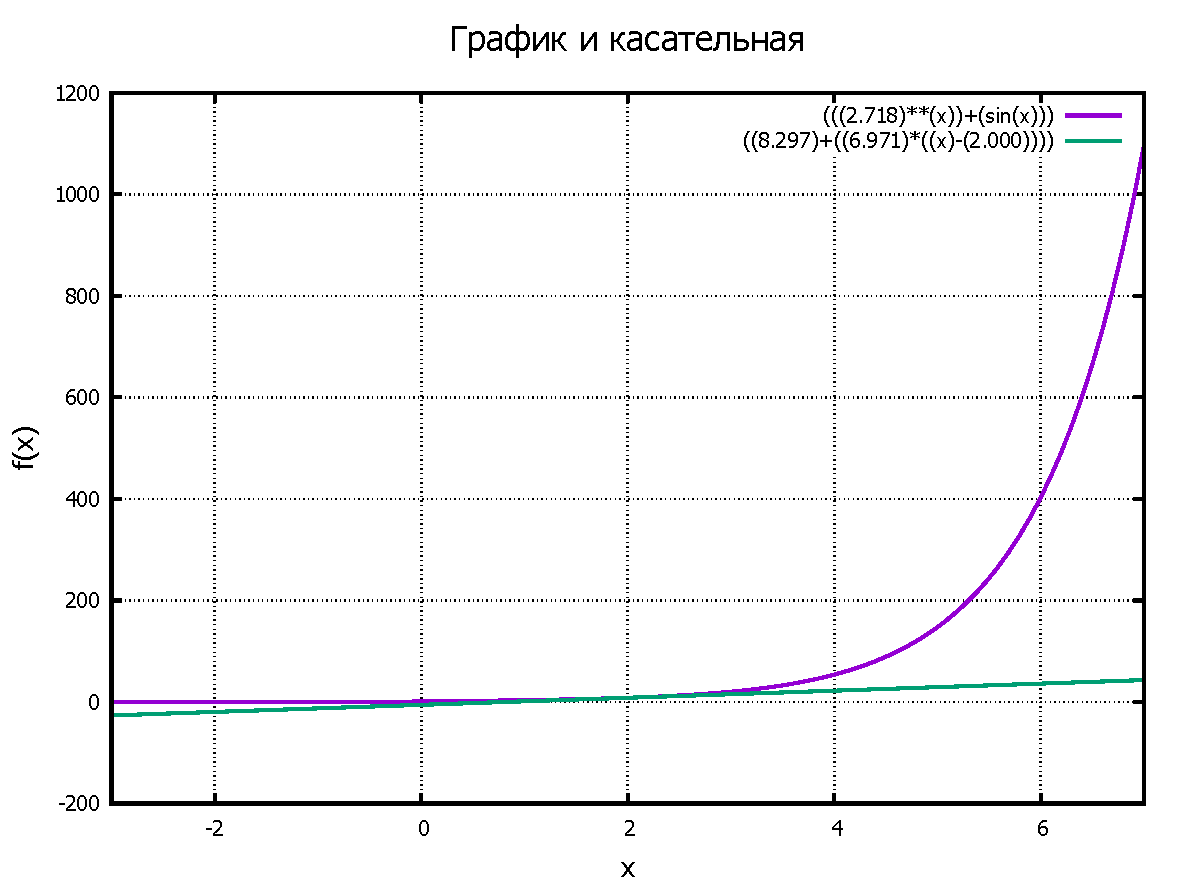
\includepdf[pages=-]{latex/graph1.pdf}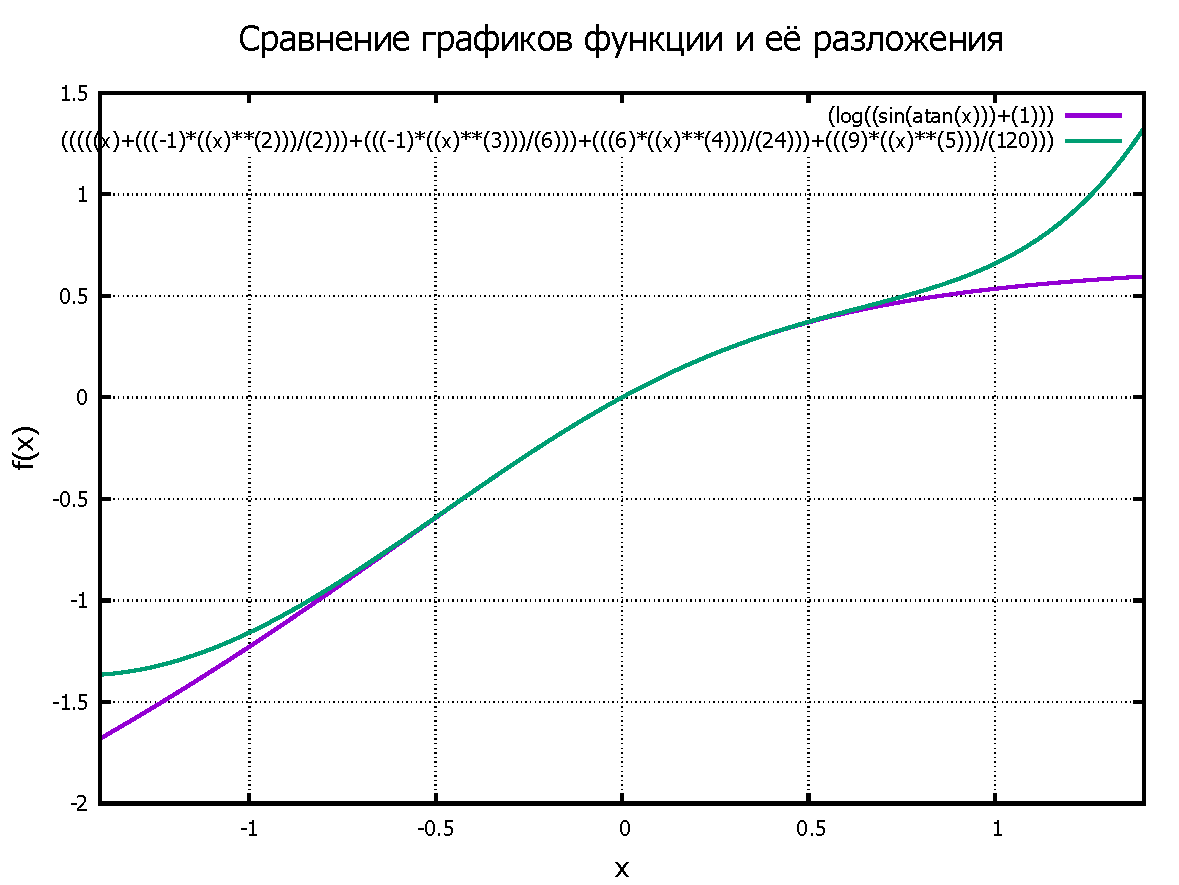
\includepdf[pages=-]{latex/graph2.pdf}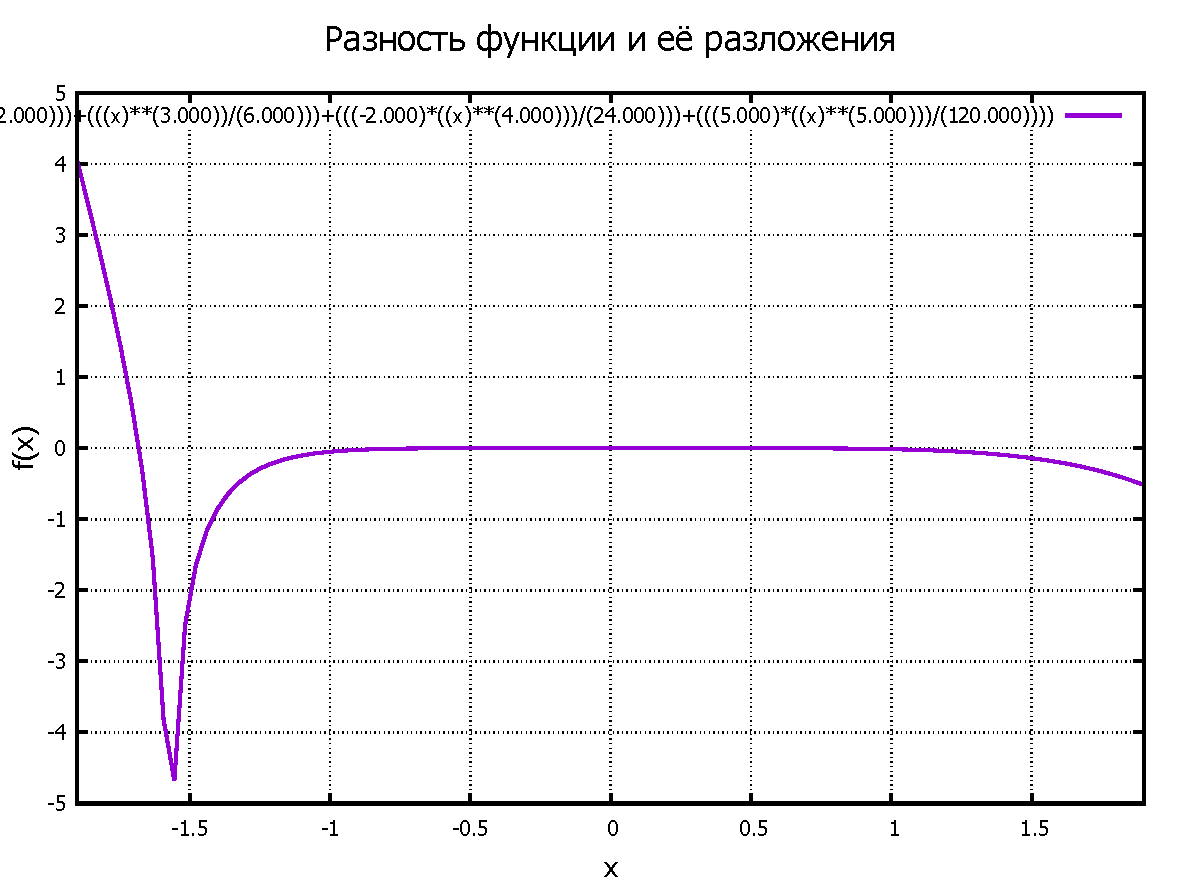
\includepdf[pages=-]{latex/graph3.pdf}\end{flushleft}
\end{document}